\subsection{遮断効果}
\label{sec:chapter5_beta_shock_insulation}
次に国際的な波及効果について考察する。
本稿のシミュレーションにおいては自国の金融政策の違いが主要な外国関連変数
\(\{\lambda_t^{H/*},\lambda_t^{F/*},p_t^{F*},i_t^F,c_t^{H\to F},c_t^{F\to F},y_t^F,l_t^F,
\bar{p}_t^{F*},\pi_t^{F*},\widetilde{p}_t^{F*},v_t^F,w_t^F,t_t^{F*},b_t^H,\Delta_t^F\}\) 
にまったく影響を与えないという結果が得られた。
これは遮断効果として知られている\parencite{ColeObstfeld1991}。
ただし完全伸縮物価IT-PPIのみグラフが異なっており、
これは価格硬直性パラメータ\(\xi^H\)が異なるためである。
遮断効果の詳しい説明は付録
\ref{sec:appendix_insulation_effect_TODO}
に記す。
\begin{figure}[H]
    \centering
    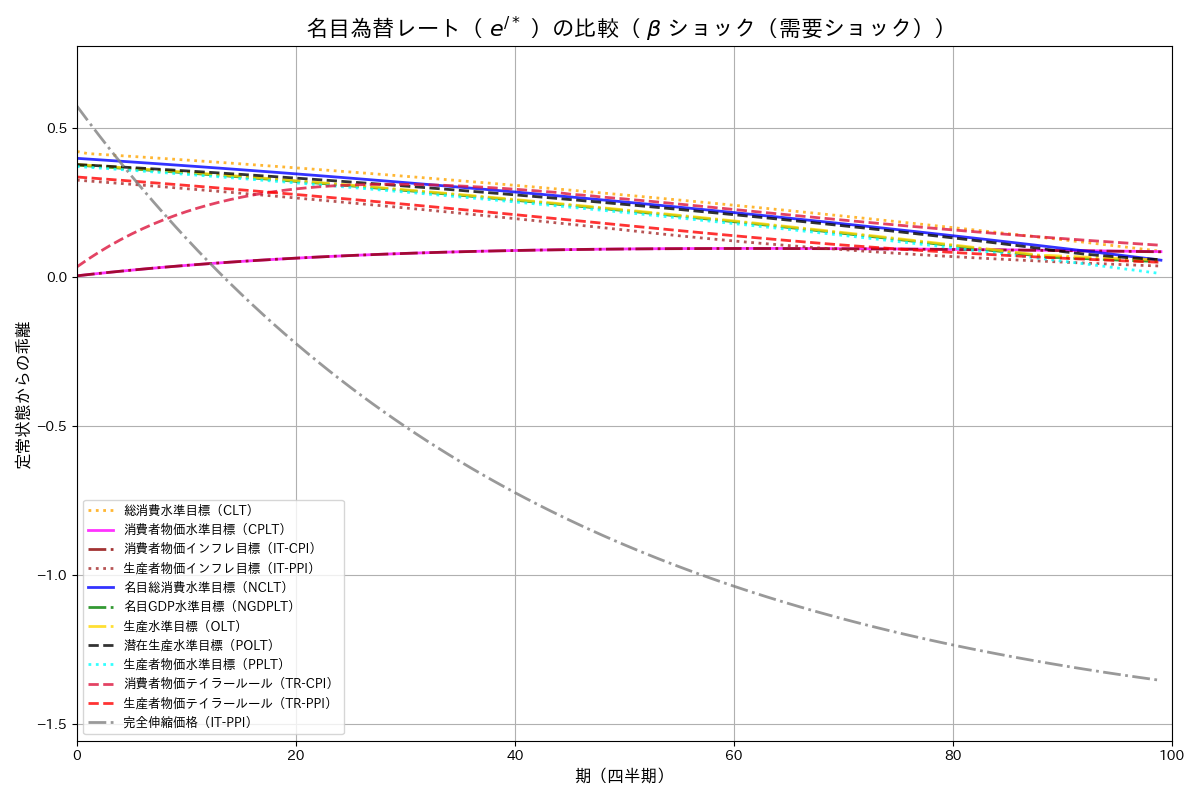
\includegraphics[width=0.9\textwidth]{comparison_graphs/beta_shock/beta_shock_e_slash_star.png}
    \caption{自国通貨建て名目為替レート（\(e^{/*}\)）}
    \label{fig:chapter5_beta_shock_insulation_e_slash_star}
\end{figure}
\begin{figure}[H]
    \centering
    \phantomcaption % 図番号を確保
    \label{fig:chapter5_beta_shock_foreign_vars}
    \makebox[\textwidth][c]{
        \begin{minipage}{1.2\textwidth}
            \centering
            \begin{subfigure}{0.48\linewidth}
                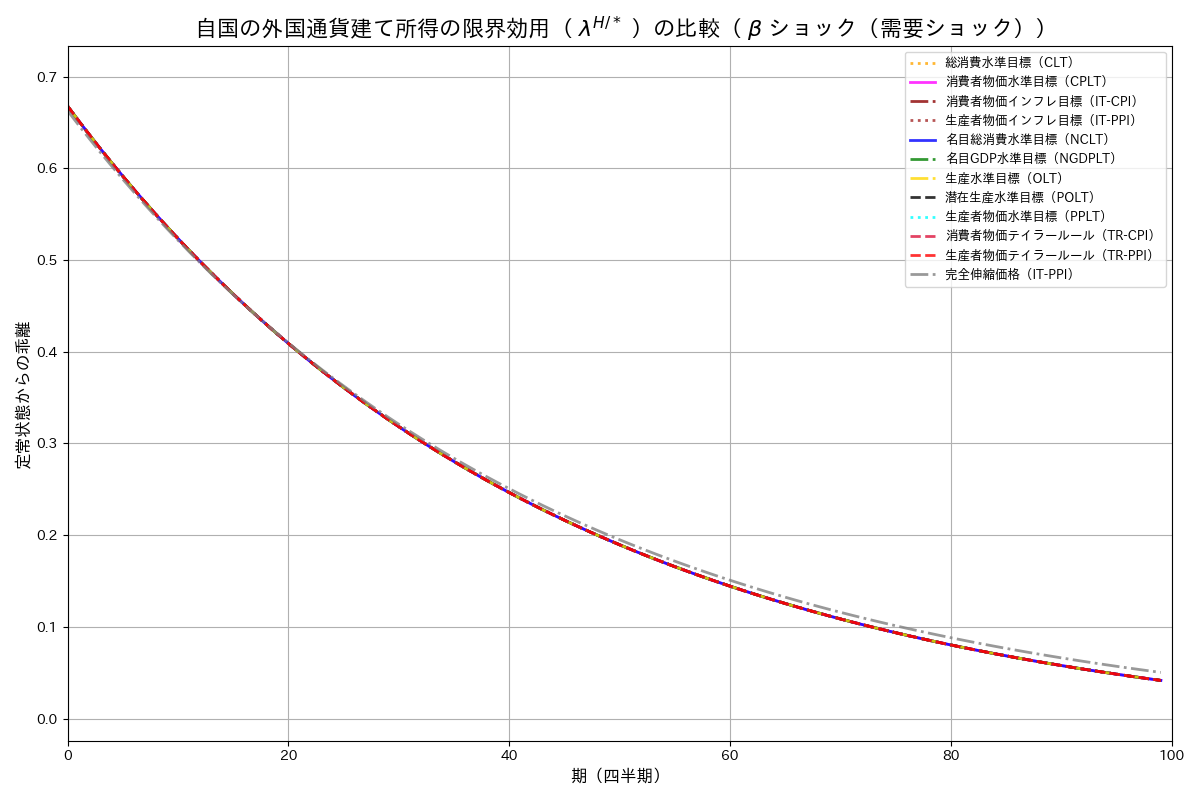
\includegraphics[width=\linewidth]{comparison_graphs/beta_shock/beta_shock_lambda_H_slash_star.png}
                \caption{自国の外国通貨建て所得の限界効用（\(\lambda^{H/*}\)）}
                \label{fig:chapter5_beta_shock_insulation_lambda_H_slash_star}
            \end{subfigure}
            \hfill
            \begin{subfigure}{0.48\linewidth}
                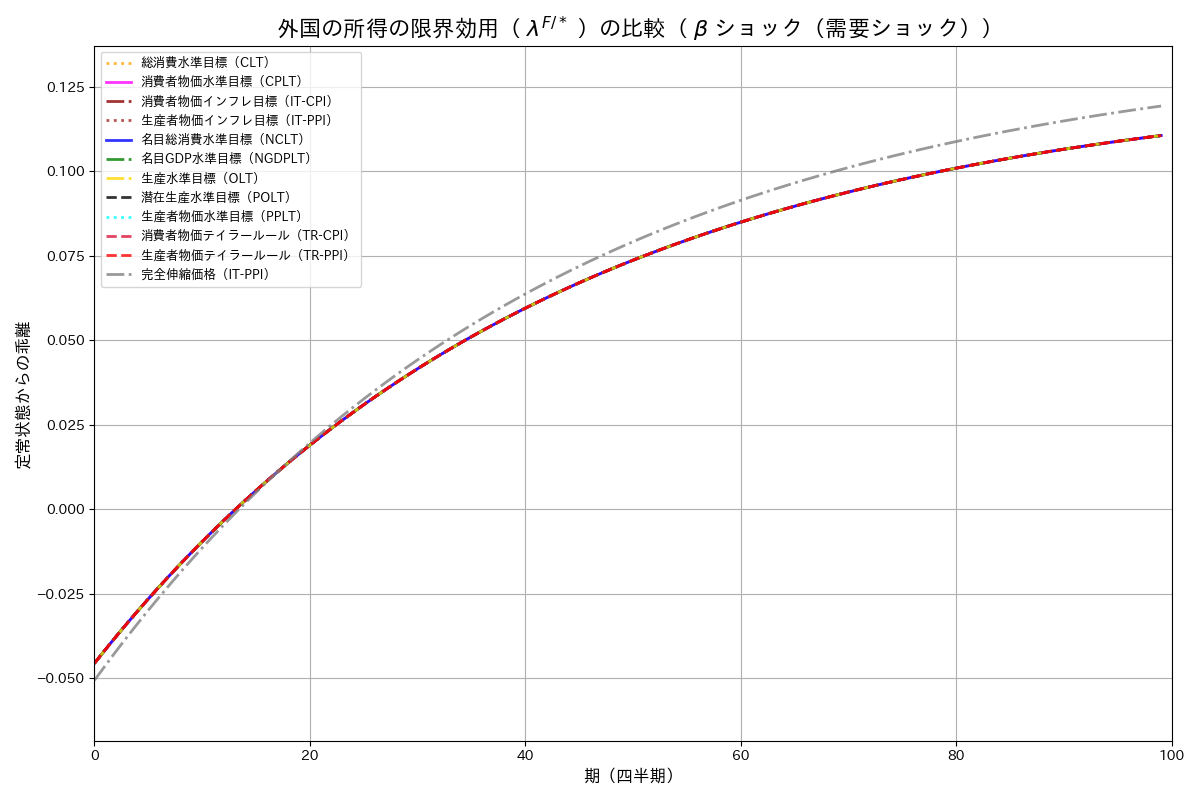
\includegraphics[width=\linewidth]{comparison_graphs/beta_shock/beta_shock_lambda_F_slash_star.png}
                \caption{外国の所得の限界効用（\(\lambda^{F/*}\)）}
                \label{fig:chapter5_beta_shock_insulation_lambda_F_slash_star}
            \end{subfigure}
        \end{minipage}
    }
\end{figure}
\begin{figure}[H]
    \ContinuedFloat
    \centering
    \makebox[\textwidth][c]{
        \begin{minipage}{1.2\textwidth}
            \centering
            \begin{subfigure}{0.48\linewidth}
                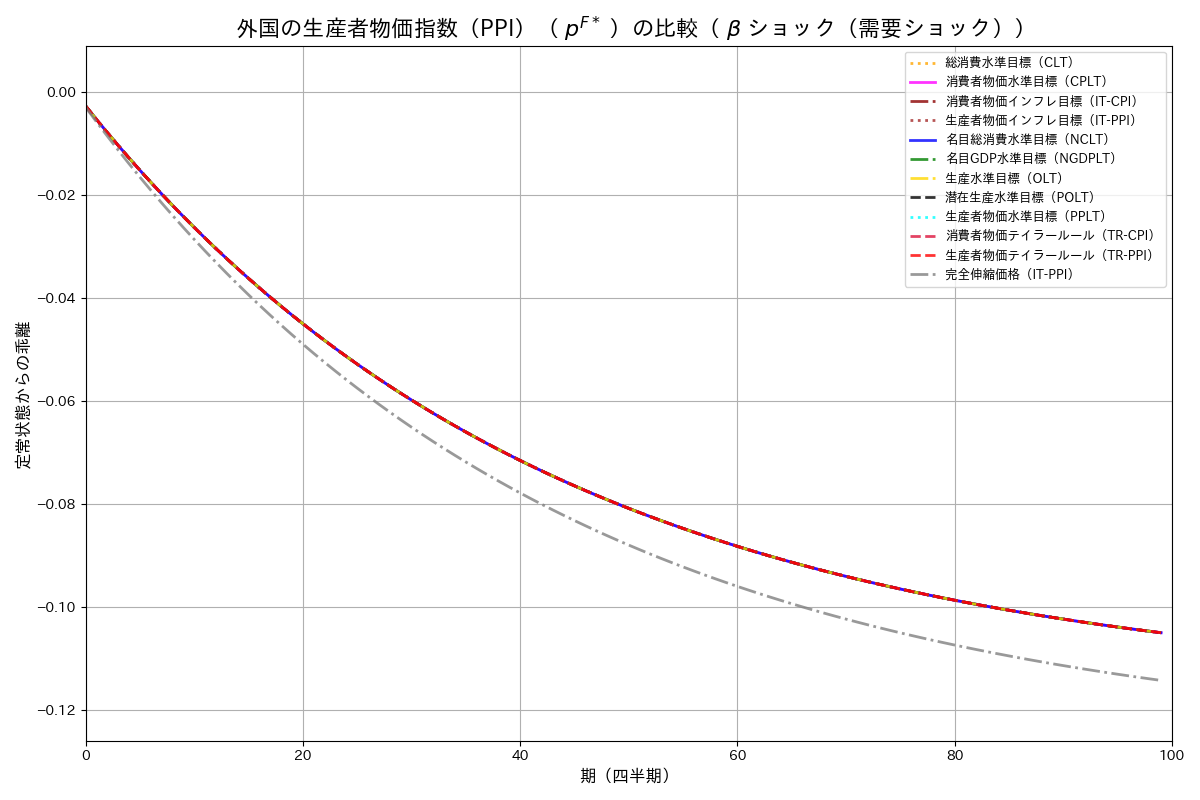
\includegraphics[width=\linewidth]{comparison_graphs/beta_shock/beta_shock_p_F_star.png}
                \caption{外国の生産者物価指数(PPI)（\(p^{F*}\)）}
                \label{fig:chapter5_beta_shock_insulation_p_F_star}
            \end{subfigure}
            \hfill
            \begin{subfigure}{0.48\linewidth}
                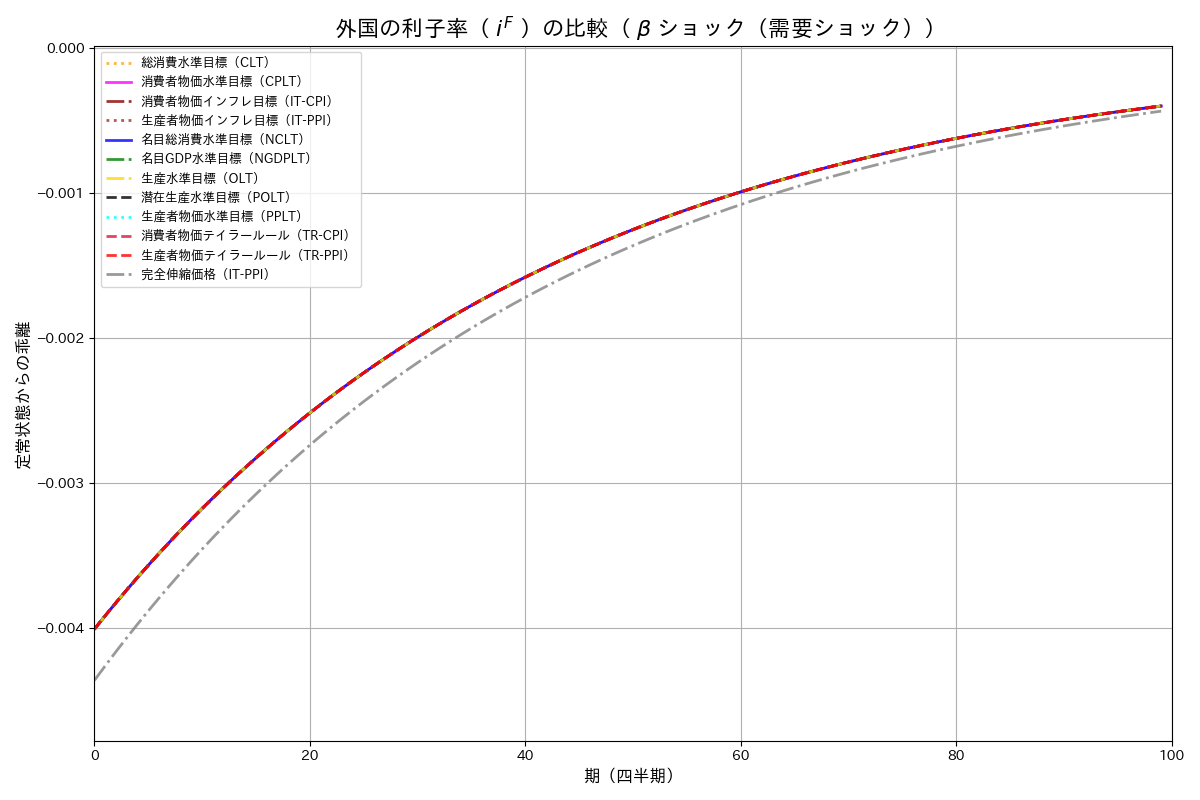
\includegraphics[width=\linewidth]{comparison_graphs/beta_shock/beta_shock_i_F.png}
                \caption{外国の名目利子率（\(i^F\)）}
                \label{fig:chapter5_beta_shock_insulation_i_F}
            \end{subfigure}
        \end{minipage}
    }
\end{figure}
\begin{figure}[H]
    \ContinuedFloat
    \centering
    \makebox[\textwidth][c]{
        \begin{minipage}{1.2\textwidth}
            \centering
            \begin{subfigure}{0.48\linewidth}
                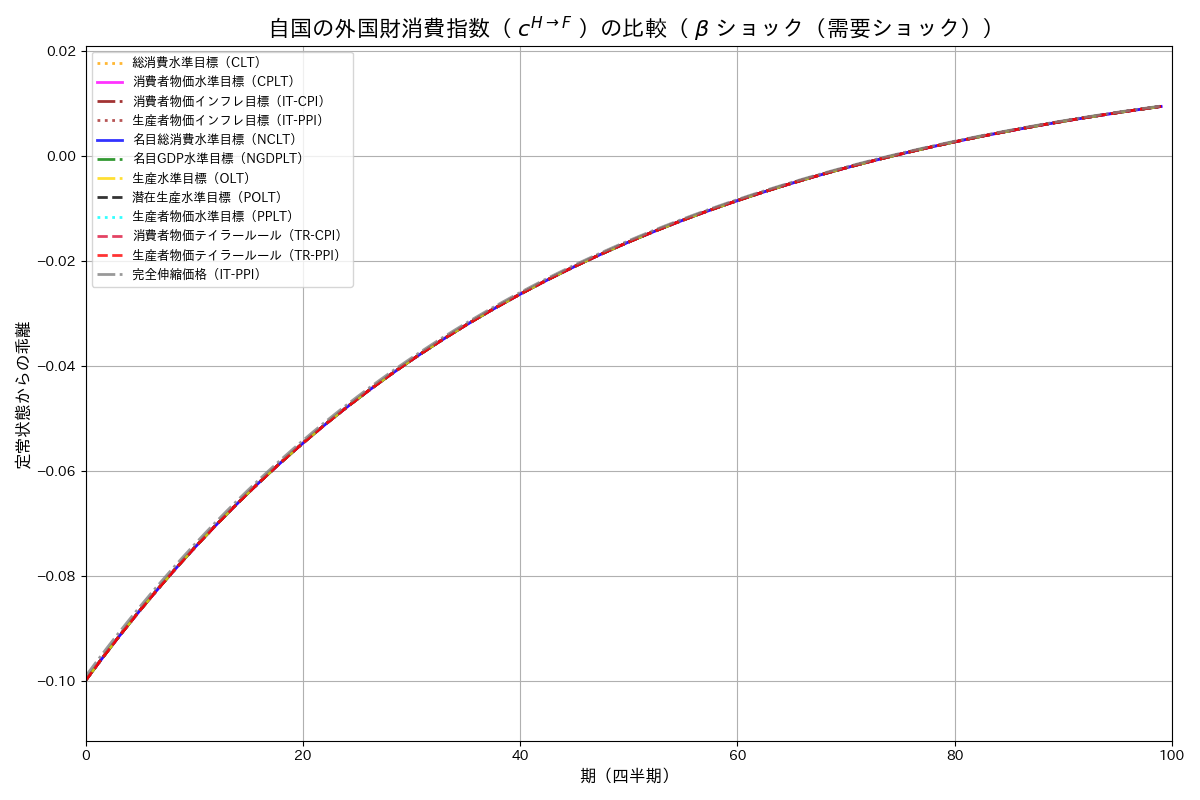
\includegraphics[width=\linewidth]{comparison_graphs/beta_shock/beta_shock_c_H_F.png}
                \caption{自国の外国財消費指数（\(c^{H\to F}\)）}
                \label{fig:chapter5_beta_shock_insulation_c_H_F}
            \end{subfigure}
            \hfill
            \begin{subfigure}{0.48\linewidth}
                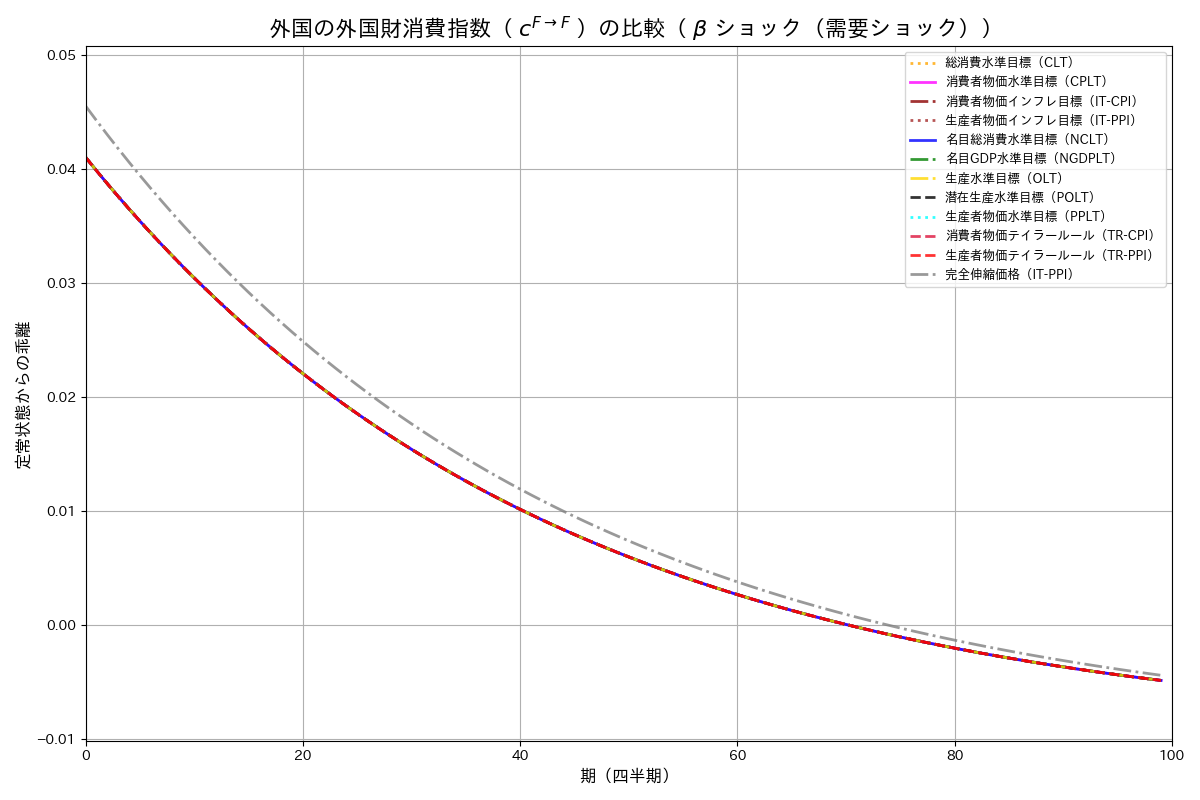
\includegraphics[width=\linewidth]{comparison_graphs/beta_shock/beta_shock_c_F_F.png}
                \caption{外国の外国財消費指数（\(c^{F\to F}\)）}
                \label{fig:chapter5_beta_shock_insulation_c_F_F}
            \end{subfigure}
        \end{minipage}
    }
\end{figure}
\begin{figure}[H]
    \ContinuedFloat
    \centering
    \makebox[\textwidth][c]{
        \begin{minipage}{1.2\textwidth}
            \centering
            \begin{subfigure}{0.48\linewidth}
                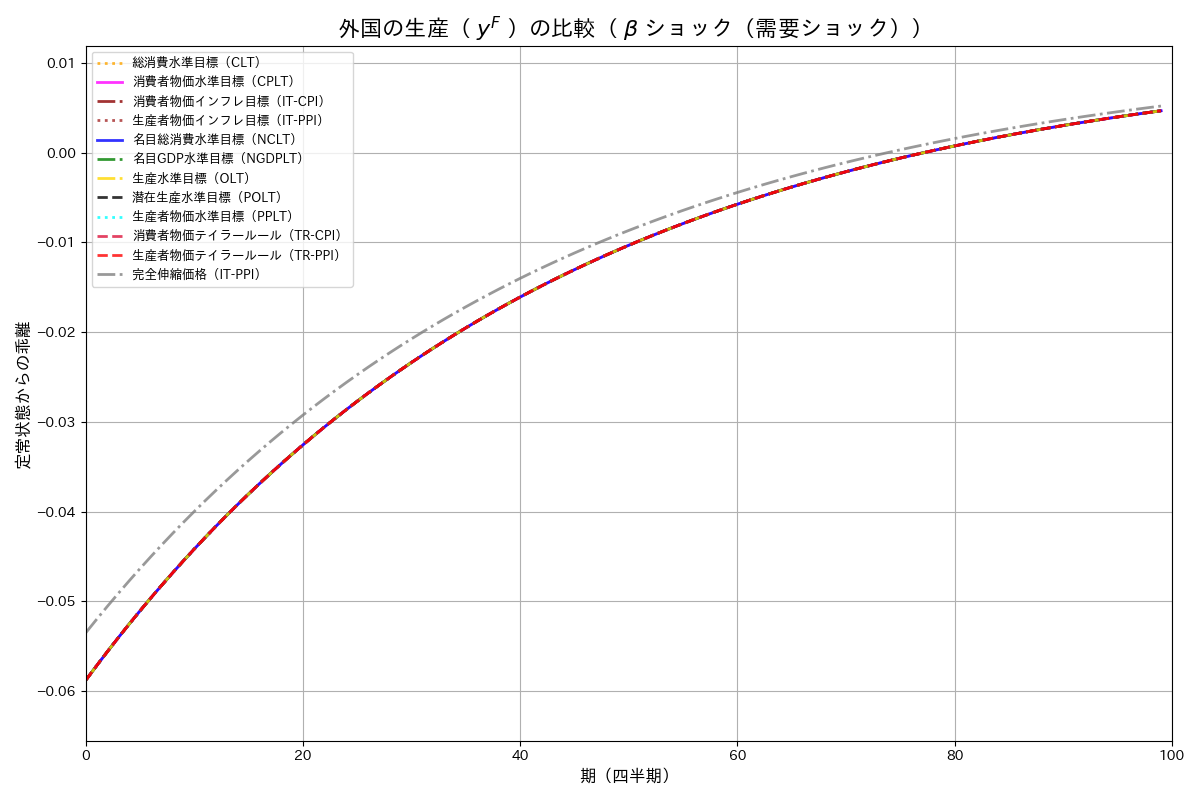
\includegraphics[width=\linewidth]{comparison_graphs/beta_shock/beta_shock_y_F.png}
                \caption{外国の生産（\(y^F\)）}
                \label{fig:chapter5_beta_shock_insulation_y_F}
            \end{subfigure}
            \hfill
            \begin{subfigure}{0.48\linewidth}
                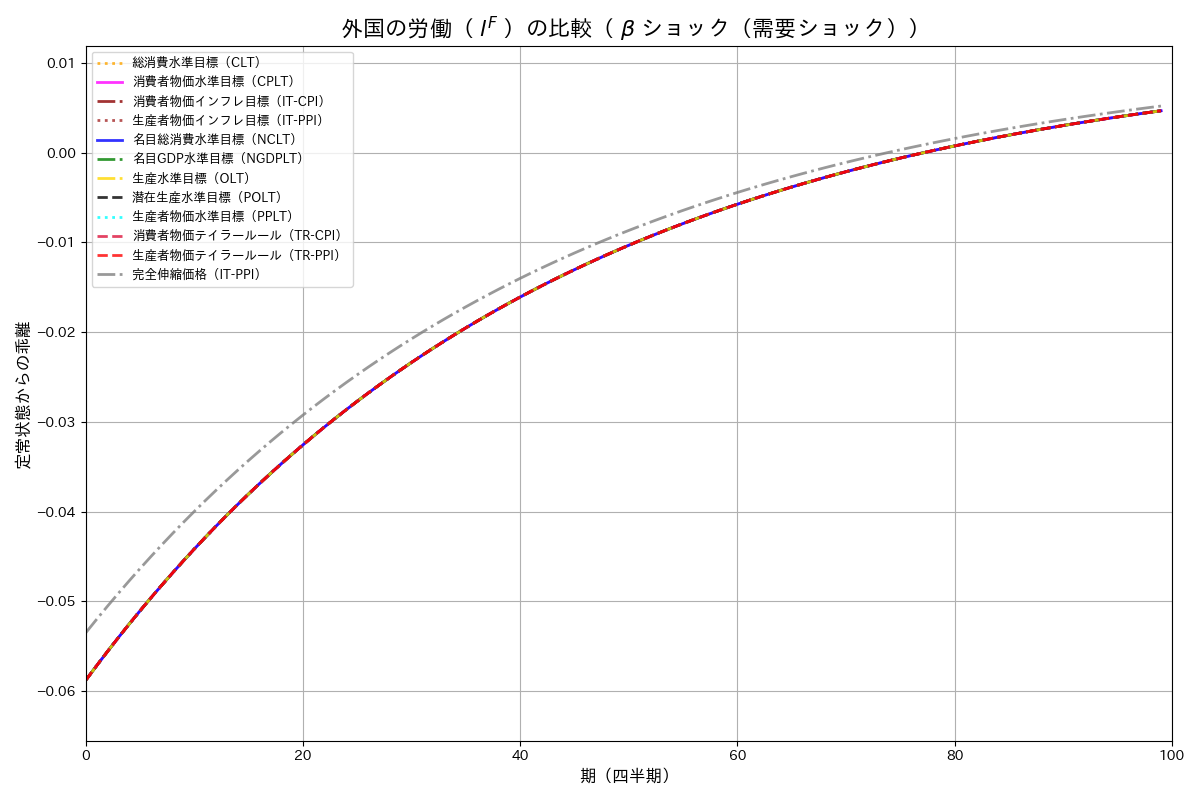
\includegraphics[width=\linewidth]{comparison_graphs/beta_shock/beta_shock_l_F.png}
                \caption{外国の労働（\(l^F\)）}
                \label{fig:chapter5_beta_shock_insulation_l_F}
            \end{subfigure}
        \end{minipage}
    }
\end{figure}
\begin{figure}[H]
    \ContinuedFloat
    \centering
    \makebox[\textwidth][c]{
        \begin{minipage}{1.2\textwidth}
            \centering
            \begin{subfigure}{0.48\linewidth}
                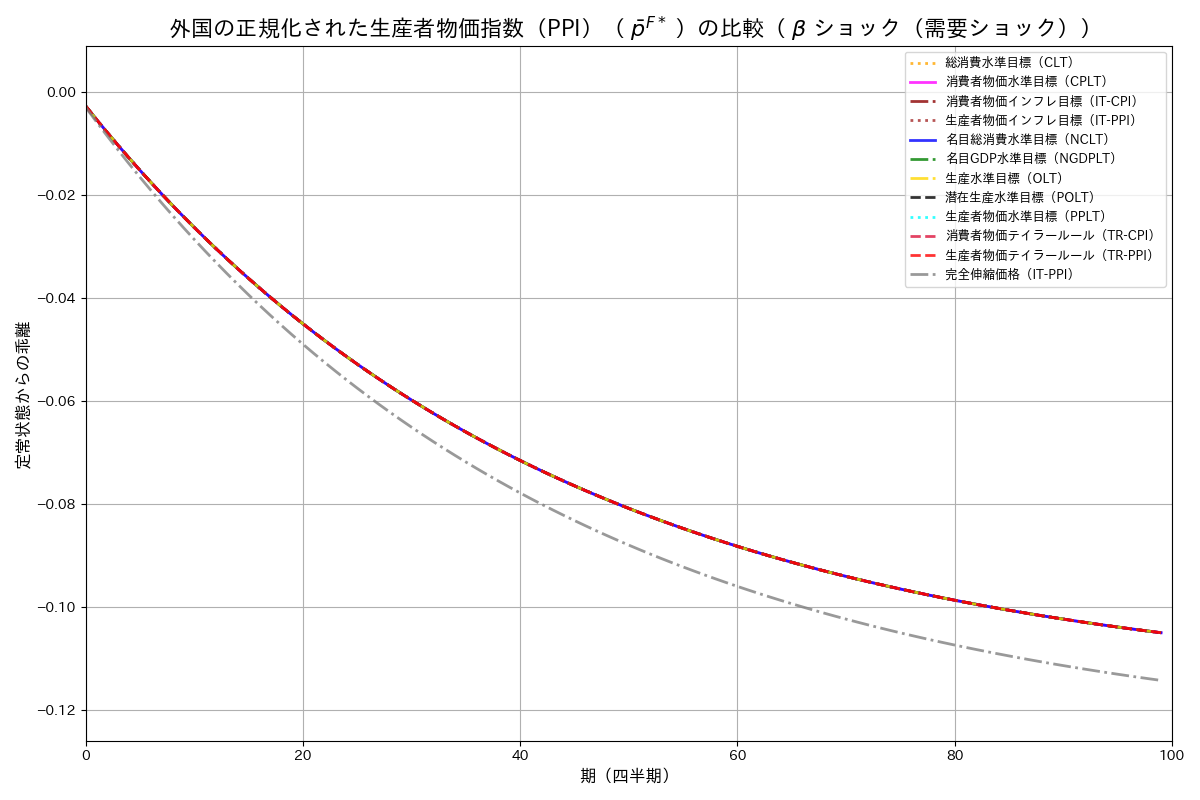
\includegraphics[width=\linewidth]{comparison_graphs/beta_shock/beta_shock_p_F_star_bar.png}
                \caption{外国の正規化された生産者物価指数(PPI)（\(\bar{p}^{F*}\)）}
                \label{fig:chapter5_beta_shock_insulation_p_F_star_bar}
            \end{subfigure}
            \hfill
            \begin{subfigure}{0.48\linewidth}
                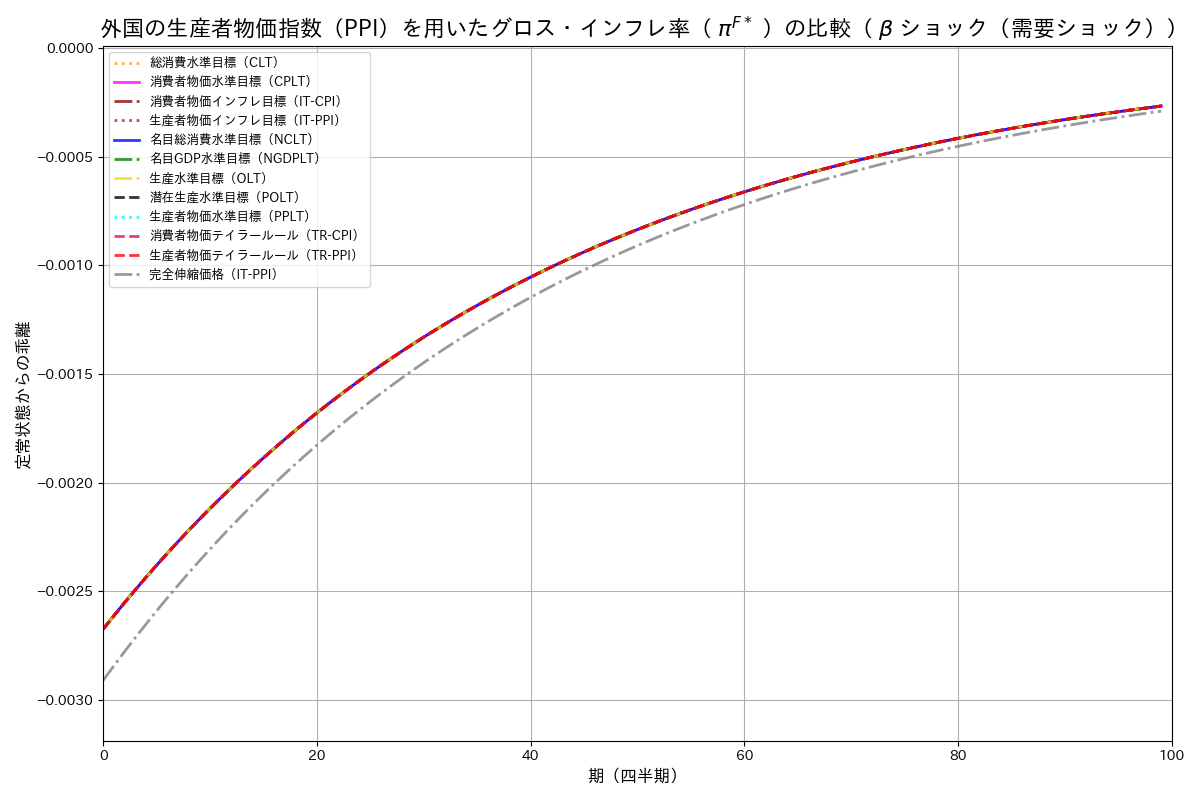
\includegraphics[width=\linewidth]{comparison_graphs/beta_shock/beta_shock_pi_F_star.png}
                \caption{外国の正規化された生産者物価指数(PPI)を用いたグロス・インフレ率（\(\pi^{F*}\)）}
                \label{fig:chapter5_beta_shock_insulation_pi_F_star}
            \end{subfigure}
        \end{minipage}
    }
\end{figure}
\begin{figure}[H]
    \ContinuedFloat
    \centering
    \makebox[\textwidth][c]{
        \begin{minipage}{1.2\textwidth}
            \centering
            \begin{subfigure}{0.48\linewidth}
                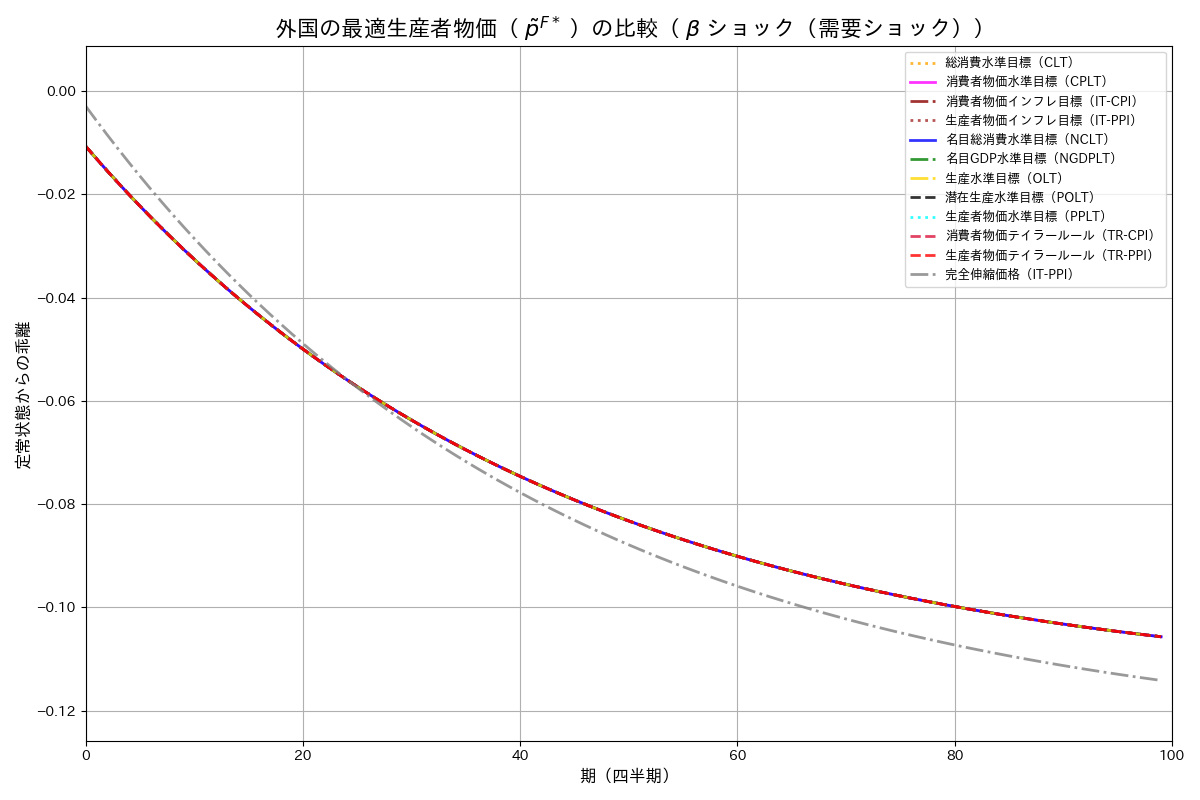
\includegraphics[width=\linewidth]{comparison_graphs/beta_shock/beta_shock_p_F_star_tilde.png}
                \caption{外国の最適生産者物価（\(\widetilde{p}^{F*}\)）}
                \label{fig:chapter5_beta_shock_insulation_p_F_star_tilde_sub}
            \end{subfigure}
            \hfill
            \begin{subfigure}{0.48\linewidth}
                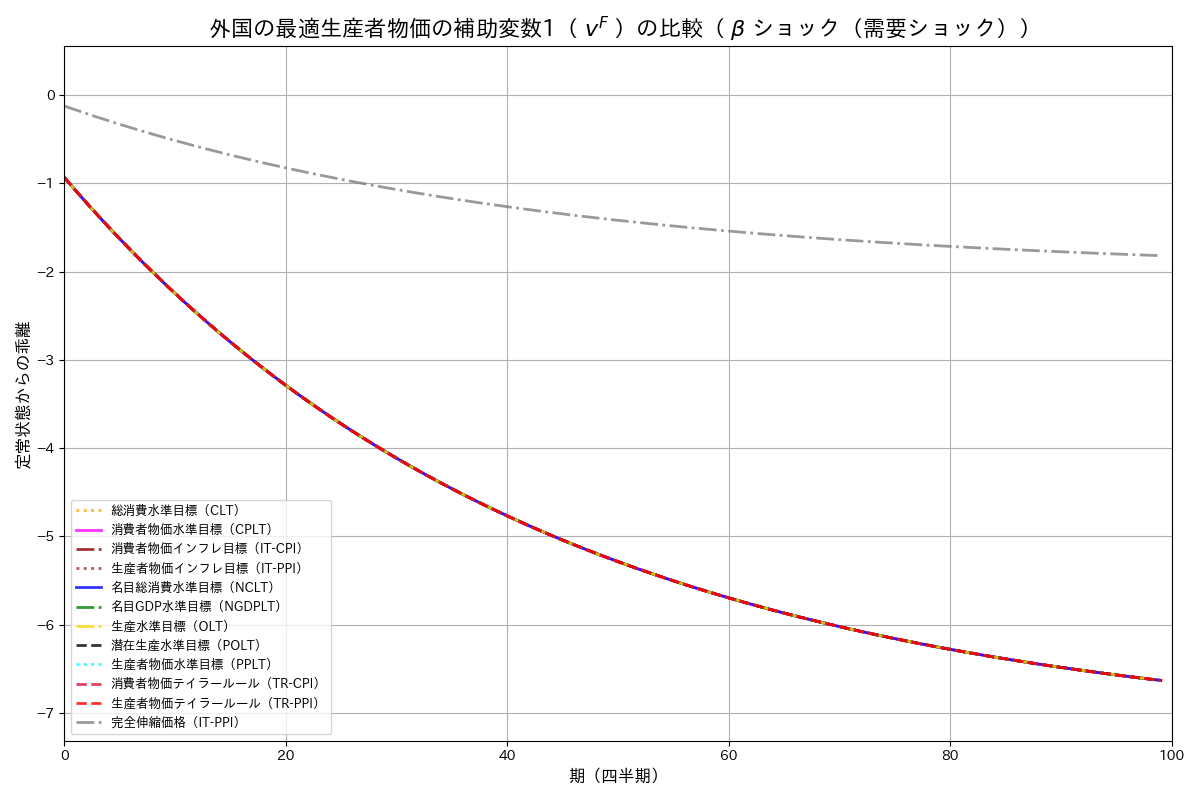
\includegraphics[width=\linewidth]{comparison_graphs/beta_shock/beta_shock_v_F.png}
                \caption{外国の最適生産者物価の補助変数1（\(v^F\)）}
                \label{fig:chapter5_beta_shock_insulation_v_F}
            \end{subfigure}
        \end{minipage}
    }
\end{figure}
\begin{figure}[H]
    \ContinuedFloat
    \centering
    \makebox[\textwidth][c]{
        \begin{minipage}{1.2\textwidth}
            \centering
            \begin{subfigure}{0.48\linewidth}
                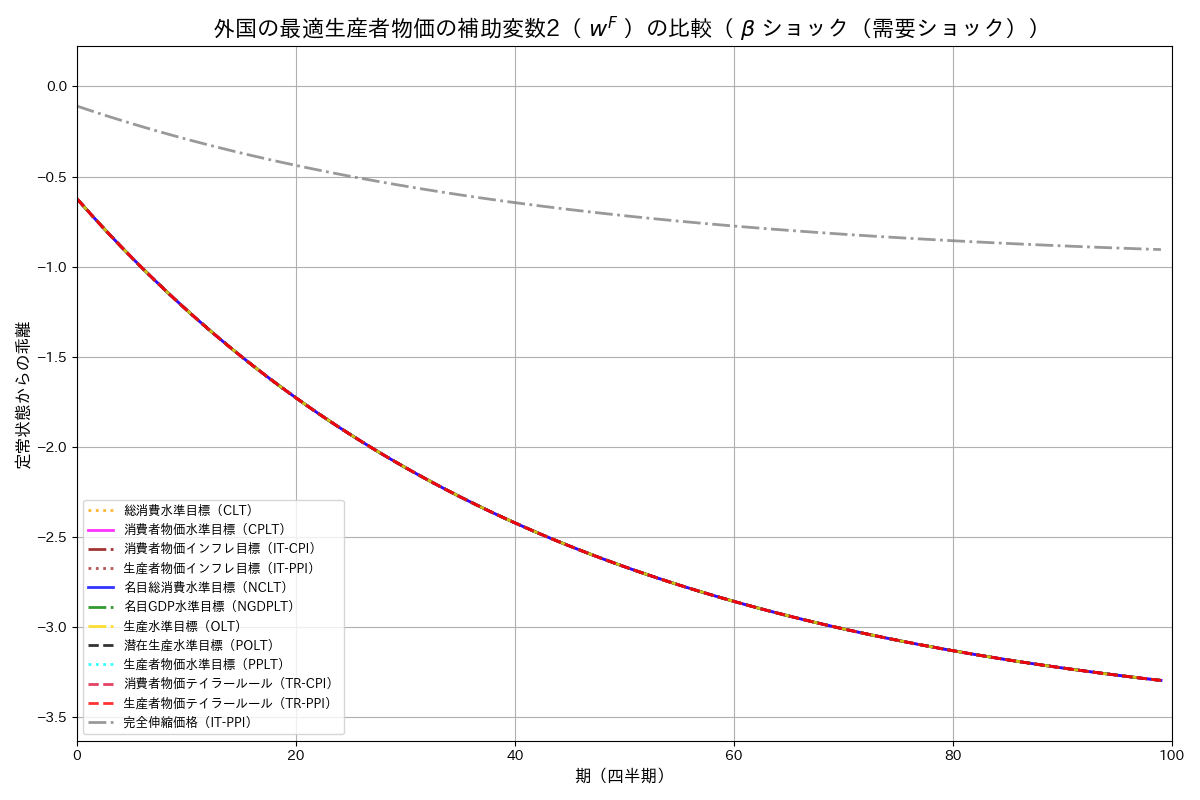
\includegraphics[width=\linewidth]{comparison_graphs/beta_shock/beta_shock_w_F.png}
                \caption{外国の最適生産者物価の補助変数2（\(w^F\)）}
                \label{fig:chapter5_beta_shock_insulation_w_F}
            \end{subfigure}
            \hfill
            \begin{subfigure}{0.48\linewidth}
                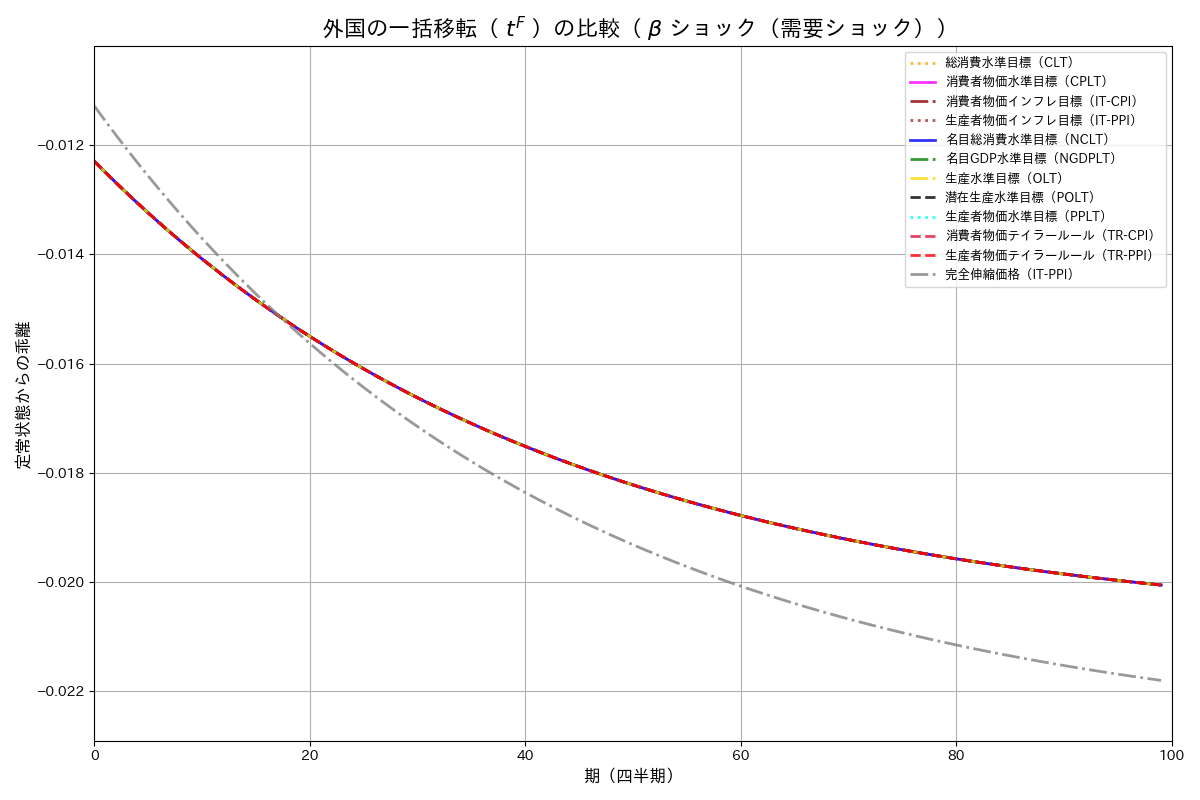
\includegraphics[width=\linewidth]{comparison_graphs/beta_shock/beta_shock_t_F.png}
                \caption{外国の一括移転（\(t^F\)）}
                \label{fig:chapter5_beta_shock_insulation_t_F}
            \end{subfigure}
        \end{minipage}
    }
\end{figure}
\begin{figure}[H]
    \ContinuedFloat
    \centering
    \makebox[\textwidth][c]{
        \begin{minipage}{1.2\textwidth}
            \centering
            \begin{subfigure}{0.48\linewidth}
                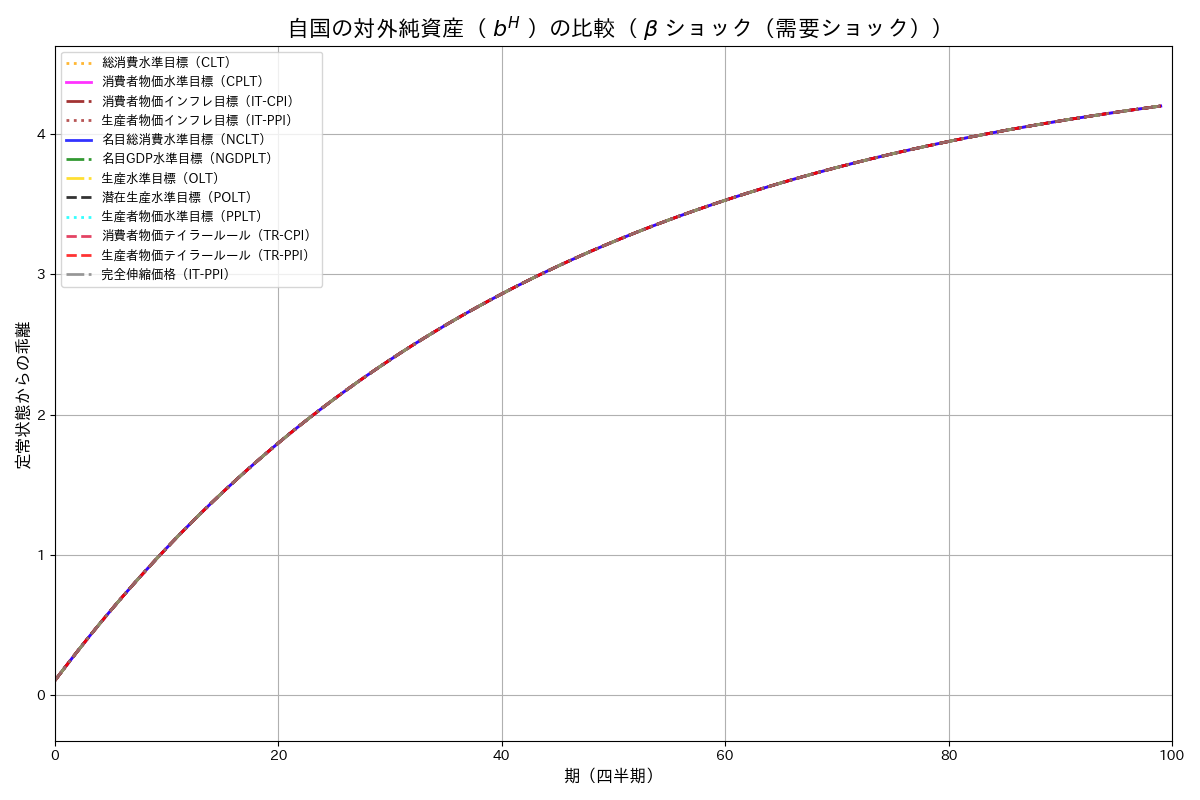
\includegraphics[width=\linewidth]{comparison_graphs/beta_shock/beta_shock_b_H.png}
                \caption{自国の対外純資産（\(b^H\)）}
                \label{fig:chapter5_beta_shock_insulation_b_H}
            \end{subfigure}
            \begin{subfigure}{0.48\linewidth}
                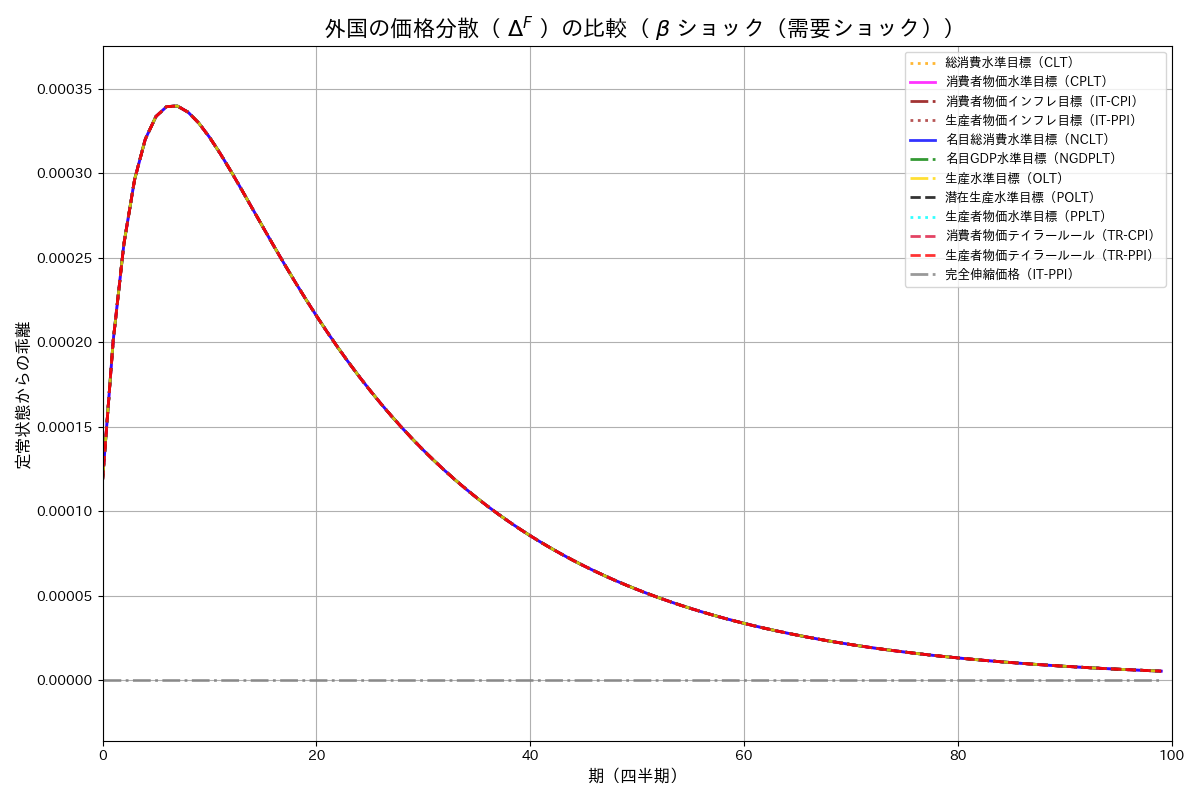
\includegraphics[width=\linewidth]{comparison_graphs/beta_shock/beta_shock_Delta_F.png}
                \caption{外国の価格分散（\(\Delta^F\)）}
                \label{fig:chapter5_beta_shock_insulation_Delta_F}
            \end{subfigure}
        \end{minipage}
    }
    % 最後にまとめてキャプションを表示
    \caption{外国経済変数のインパルス応答関数（全政策で不変）}
\end{figure}

\subsection{二平面分析}
\label{sec:chapter5_beta_shock_asad}
本節では効用や為替レートも含む主要な自国関連変数のグラフを掲載し、
各金融政策についてその効果をAS-AD分析により解釈する。
本モデルは独占的競争モデルであるため初期定常状態において経済活動が社会的に最適な水準よりも不足している。
そのため総消費指数\(c_t^{H \to W}\)や生産\(y_t^H\)が初期定常状態の水準を超えて上昇するにしたがい、
効用\(u_t^H\)も初期定常状態の水準を超えて上昇している。
こうした経済のオーバーシュートはあまりに過度であると効用\(u_t^H\)を急激に下落させることが知られているが、
効用\(u^H\)の図
\ref{}
に急激な下落は見られず、したがって過度なオーバーシュートは起こっていないことがわかる。